\documentclass[a4paper, 11pt]{article}

\usepackage[ngerman]{babel}
\usepackage[utf8]{inputenc}
\usepackage{graphicx}
\usepackage{tabularx}
\usepackage{array}
\usepackage{pbox}
\usepackage{color}
\usepackage{booktabs}
\usepackage{hyperref}
\usepackage{lmodern}

\title{Named Entity Classification}
\author{Madita Huvar, Phillip Richter-Pechanski, Sanaz Safdel}
\date{\today}

\begin{document}
\maketitle
\newpage
\tableofcontents
\newpage
\section{Einführung}
Named Entity Recognition ist seit den 1990er Jahren ein aktives Forschungsfeld. Es stellt die Grundlage für weitere Forschungsfelder zum Beispiel im Bereich Semantic Annotation, Question Answering, usw. dar.
\subsection{Was sind Named Entities?}
Named Entities sind Phrasen, die Namen von Personen, Organisationen, Währungen, usw. enthalten. In unserem Projekt werden sie wie folgt dargestellt:
%\begin{exampleblock}{Beispiele für Named Entities}
%		The Speaker of the [ORG U.N.] .. \newline 
%		President [PER Obama] ... \newline 
%		The price of the [MONEY Dollar] lost ... \newline
%		[LOC Moscow] is the capital of Russia. 
%\end{exampleblock}
\section{Unser Projekt}
\subsection{Ziel}
Typischerweise werden Named Entity Recognition und Named Entity Classification zusammen betrachtet und nur wenige Untersuchungen beschäftigen sich nur mit Named Entity Classification. In unserem Projekt konzentrieren wir uns auf Named Entity Classification und stellen vor allem die Frage, welchen Einfluss Feature Selection auf die Klassifikationsergebnisse eines Named Entity Klassifizierers haben. Wir verwenden hierzu einfache syntaktische und lexikalische Features, die in fast allen Forschungsarbeiten in ähnlicher Form genutzt werden.
\subsection{Organisation}
Zur Organisation unseres Projekts benutzen wir GitHub. Zusätzlich haben wir eine WhatsApp Gruppe, in der wir uns besprechen und unsere Treffen planen können. Diese finden ca. ein bis zwei Mal pro Woche statt. Unsere Ergebnisse halten wir auf einer speziell angelegten Wikiseite fest. 
\section{Tools}
Für unser Projekt verwenden wir folgende Tools:
\begin{itemize}
\item Python 3.4+
\item Scikit Learn (als Klassifizierer)
\item liac-arff
\item matplotlib
\item Weka (zur Korpusanalyse)
\item GitHub
\item ICL-Wiki
\end{itemize}
\section{Korpus & Korpusklassen}
\subsection{Korpus}
Wir verwenden für unser Projekt das OntoNotes Korpus 2012. In diesem sind englische Nachrichtentexte des 'The Wall Street Journal' enthalten. Es existieren bereits ein Development-/Trainings- und Testset. Siehe Tabelle \ref{tab:datasets}.
\subsection{Korpusreader}
Für die Extraktion der Named Entities haben wir einen Korpusreader erstellt. Dieser Reader extrahiert alle Named Entities, inklusive POS-Tags der einzelnen Token, Phrasenart und Kontextwörter (ne-1, ne+1) und ordnet ihnen Klassen zu.
\subsection{Korpusklassenbalancierung}
Die Anzahl der Named Entites im Trainingsset ist für die einzelnen Klassen sehr unterschiedlich, wie in Tabelle \ref{tab:klassenOntoNotes} zu sehen. Die zehn Klassen mit der geringsten Anzahl Named Entities, werden aus dem balancierten Korpus entfernt. Die Klassen NORP und GPE werden zusammengefasst, da sie semantisch ähnlich sind. Die numerischen Klassen MONEY, PERCENT und CARDINAL werden ebenfalls zusammengefasst.
Daraus ergeben sich unsere neuen Korpusklassen, zu sehen in Tabelle \ref{tab:balancierteKlassen}.
Die Verteilung der Named Entities auf die Klassen ist nun wesentlich ausgeglichener, wie in Tabelle \ref{tab:VerteilungKlassen} zu sehen.
\section{Baselineklassifizierer}
Für unseren Baselineklassifizierer verwenden wir nur das Feature 'Unigram', welches die Vorkommenshäufigkeit, der Unigramme in der Named Entity, welche mindestens fünfmal im Trainigskorpus vorkommen, beschreibt.
\section{Erweiterter Klassifizierer}
\subsection{Erweitertes Featureset}
Für unseren Named Entity Klassifizierer, haben wir weitere Features hinzugefügt. Diese sind in Tabelle \ref{tab:allf1} beschrieben. Insgesamt hatten wir eine Anzahl von 1716 Features.
\subsection{Klassifizierertyp}
Zur KLassifizierung der Named Entities wir eine Support Vector Maschine mit linearem Kernel verwendet. SVM XXXXXXFOLIEN
Unsere Featurevektoren haben sehr viele Features, daher verwenden wir den linearen Kernel. Mapping in höheren Featurespace eines nicht-linearen Kernels bringt kaum Klassifiziereungsverbesserungen. Alernativ haben wir Decisiontree getestet, dieser hatte allerdings mit allen Featurekombinationen tendenziell schlechtere Evaluationsergebnisse. Zudem trainiert der SVM deutlich schneller. Dies wird deutlich in Abbildung \ref{img:roccurve} und Abbildung \ref{img:matrix}
\section{Featureselection}
Insgesamt wurden elf Features eingesetzt. Um die Performance der einzelnen Features zu testen, wurde die Potenzmenge des Featuresets gebildet. Schließlich wurde der Klassifizierer auf allen 1013 Teilmengen durchgeführt. Für die Evaluation entscheidend waren alle Teilmengen, die die Features 'Unigram' und 'Context' enthalten und mindestens drei Features besitzen. Die Accuracy ohne diese Features lag nur bei <69\%. Wohingegen die Accuracy nur mit den Features 'Unigram' und 'Context' bei 87.42\% lag. Wie in Abbildung \ref{img:canvas} zu sehen erreichen wir die höchste Accuracy ab sieben Features. Jedoch schon ab vier Features gibt es kaum noch Verbesserungen der Accuracy. Die Features, die zur Erhöhung der Accuracy beitragen sind: 'POS', 'is_all_caps', 'is_in_wiki', 'is_np' und 'contains_digit'. Die beste Accuracy bei möglichst kleinem Featureset erreichen wir mit 'Unigram', 'Context', 'POS', und 'is_all_caps'.
\section{Evaluation}
Insgesamt haben wir unsere Baseline deutlich geschlagen. Sowohl mit dem balancierten, als auch mit dem unbalancierten Datenset, konnten wir bessere Ergebnisse erzielen, als unsere Baseline. Die Ergebnisse sind in Tabelle \ref{tab:Evaluation} zu sehen.
\subsection{Probleme und Lösungsvorschläge}
Während des Projekts sind wir auf einige Probleme gestoßen. Einige davon könnten mit mehr Zeit/Aufwand sicherlich gelöst werden. Ein mögliches Problem ist, dass das OntoNotes Korpus bereits automatisch annotiert ist und dadurch bereits vor unserer Verarbeitung Klassifikationsfehler im Testset vorhanden sind. Um dieses Problem zu beheben, müsste man das Korpus Handannotieren, was jedoch sehr aufwändig ist. Die Klassifizierung der Klasse PERSON könnte möglicherweise durch die Generierung weiterer PERSON-Instanzen verbessert werden. Ein weiterer Punkt, den man genauer betrachten könnte, ist das Feature 'Context', dieses bezieht um Moment auch Satzzeichen mit ein. Man könnte testen, ob eine Verbesserung erzielt wird, wenn man das Feature auf alphanumerische Strings beschränkt.
\section{Zusammenfassung}
In unserem Projekt haben wir herausgefunden, dass mehr Features nicht zwangsläufig bessere Ergebnisse liefern. Außerdem scheint die Dimensionalität der Features Einfluss auf die Klassifikationsergebnisse zu haben. Hochdimensionale Features wie 'Unigram' oder 'Context' tragen maßgeblich zu besseren Ergebnisse bei. Auch das Zusammenfassen von Klassen, die sich ähneln verbessert die Ergebnisse.
\newpage
\section{Anhang}
\begin{table}
	\begin{tabular}{ccc}
	\toprule
	Developmentset & Trainingset & Testset\\
	\midrule
	3325 & 23686 & 2996\\
	\bottomrule
	\end{tabular}
	\caption{Anzahl an  Named Entities}
	\label{tab:datasets}
\end{table}
\begin{table}
\begin{tabularx}{\textwidth}{Xc}
					\toprule
					Klassen  & Trainingset \\
					\midrule
					ORG  & 5788 \\
					DATE & 4080  \\
					PERSON & 3756 \\
					GPE & 3601 \\
					CARDINAL & 1852 \\
					MONEY & 1509  \\
					NORP & 1484 \\
					PERCENT & 1061  \\
					FAC, LOC, PRODUCT, EVENT, WORK\_OF\_ART, LAW, LANGUAGE, TIME, QUANTITY, ORDINAL & $<$ 1800 \\
					\bottomrule
\end{tabularx}
\caption{Klassen im OntoNotes Korpus \textit{(OntoNotes Release 5.0 2012)}}
\label{tab:klassenOntoNotes}
\end{table}
\begin{table}
			\begin{tabularx}{\textwidth}{lX}
				\toprule
				Klassen  & Beschreibung \\
				\midrule
				PERSON 	& People, including fictional \\
				NORP\_GPE &	Nationalities or religious or political groups;
				Countries, cities, states\\
				ORGANIZATION &	Companies, agencies, institutions, etc.\\
				DATE &	Absolute or relative dates or periods\\
				PERCENT\_MONEY\_CARDINAL &	Percentage (including “\%”);
				Monetary values, including unit;
				Numerals that do not fall under another type \\
				\bottomrule
			\end{tabularx}
			\caption{Balancierte Klassen}
			\label{tab:balancierteKlassen}
\end{table}
 \begin{table}
			 	 \resizebox{\textwidth}{!}{%
			 	\begin{tabular}{lccc}
			 		\toprule
			 		Klassen  & Developmentset & Trainingset & Testset \\
			 		\midrule
			 		ORG  & 930 & 5857 & 859 \\
			 		GPE\_NORP & 732 & 5134 & 588 \\
			 		PERCENT\_CARDINAL\_MONEY & 564 & 4672 & 529 \\
			 		DATE & 613 & 4254 & 601 \\	 		
			 		PERSON & 486 & 3759 & 413 \\
			 		\bottomrule
			 	\end{tabular}}
			 	\caption{Verteilung der Klassen nach Balancierung}
			 	\label{tab:VerteilungKlassen}
\end{table}
\begin{table}
 				\begin{tabularx}{\textwidth}{llX}
 					\toprule
 					Feature & Wert & Beschreibung\\
 					\midrule
 					Unigram & numerisch & Häufigkeit der Unigramme (lemmatisiert), die mindestens fünfmal im Trainingscorpus vorkommen. \textit{(Mayfield, McNamee 2003)} \\
 					POS & numerisch  & Häufigkeit von 36 POS-Tags aus der Penn Treebank \textit{(Chieu 2003)} \\
 					isAllCaps & boolean & Wörter nur in Großschreibung \textit{(Nadenau, Turney 2006)} \\
 					Context & numerisch & Häufigkeit der Kontexttokens. Beinhaltet Vorgänger- und Nachfolgetoken der NE. \textit{(Munro, Ler 2003)}  \\
 					containsDigit & boolean & Vorkommen von Nummern. \textit{}\\
 					isInWiki & boolean & Vorkommen der NE in der Wikipedia. \textit{(Toral, Munoz 2006)} \\
 							isTitle & boolean & Prüft, ob Titelbezeichnungen (z.B. Mr., MA) vorkommen. \textit{(Ratinov, Roth 2009)} (0)\\
 							isNP & boolean & Ist NE eine Nominalphrase. \textit{(Sánchez, Cuadrado 2009)} \\
 							isName & boolean & Prüft, ob Vornamen vorkommen.\textit{(Ratinov, Roth 2009)} \\
 							containsDash & boolean & Vorkommen von Viertelgeviertstrichen. \textit{(Mayfield, McNamee 2003)}  \\
isComName & boolean & Prüft auf kommerzielle Bezeichner (Corp., Inc.) \\
 					\bottomrule
 				\end{tabularx}
 				\caption{Features für den Klassifizierer}
 				\label{tab:allf1}
\end{table}
\begin{figure}
	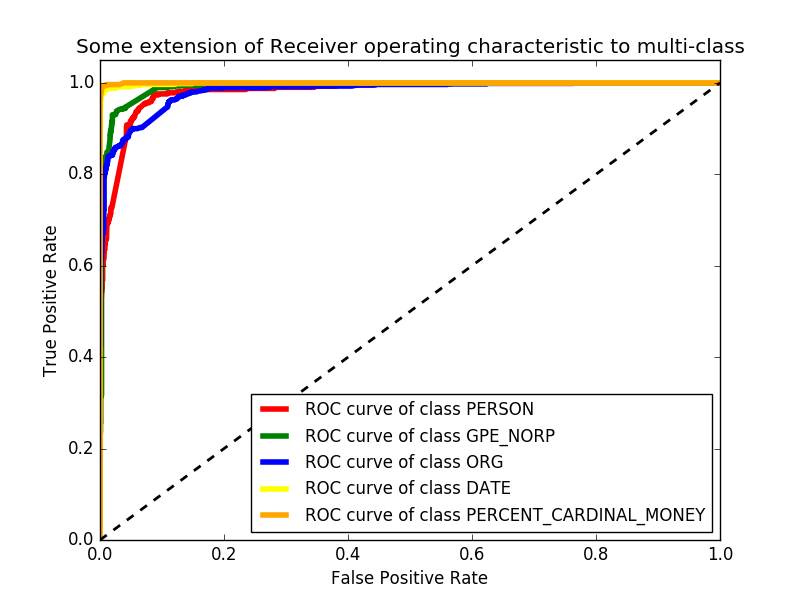
\includegraphics[scale=0.5]{roc_curve.png}
	\caption{ROC Curve}
	\label{img:roccurve}
\end{figure}
%begin{table}
%				\begin{tabularx}{\textwidth}{llllll}
%					\toprule
%					361 & 28 & 22 & 2 & 0 & PERSON\\
%					29 & 549 & 10 & 0 & 0 & GPE\_NORP\\
%					71 & 45 & 736 & 6 & 1 & ORG\\
%					0 & 2 & 1 & 591 & 7 & DATE\\
%					0 & 2 & 0 & 2 & 525 & PERCENT\_CARDINAL\_MONEY\\
%					\bottomrule
%				\end{tabularx}
%				\caption{Confusion Matrix}
%				\label{tab:matrix}
%\end{table} 
\begin{figure}
	\includegraphics[scale=0.2]{canvas.png}
	\caption{}
	\label{img:canvas}
\end{figure}
\begin{table}
					\centering
					\begin{tabular}{llll}
						Featureset & & Accuracy\\
						\toprule
						Baseline & unbalanced & 0.7867\\
						\small\color{blue}\textit{'unigram'} & balanced & 0.8408\\
						Optimales Featureset	 & unbalanced & 0.8728\\
						\small\color{blue}\textit{'pos', 'is\_all\_caps', 'is\_in\_wiki', 'is\_np', 'contains\_digit', 'unigram', 'context'}		 & balanced & 0.9237\\
						\bottomrule
					\end{tabular}
					\caption{Final Evaluation}
					\label{tab:Evaluation}
\end{table}
\end{document}
